\documentclass[12pt,oneside]{memoir} 

% Paket koji definiše sve specifičnosti master rada Matematičkog fakulteta
\usepackage[latinica,biblatex]{matfmaster} 
\usepackage{csquotes}
\usepackage{listings}
\usepackage{caption}
\usepackage[cache=false]{minted}
\usemintedstyle{monokai}

\usepackage{xcolor}

% Podrazumevano pismo je ćirilica.

% Datoteka sa literaturom u BibTex tj. BibLaTeX/Biber formatu
\bib{teza} 

% Ime kandidata na srpskom jeziku (u odabranom pismu)
\autor{Nemanja Subotić}
% Naslov teze na srpskom jeziku (u odabranom pismu)
\naslov{Programski jezici Elm i Elixir u razvoju studentskog veb portala}
% Godina u kojoj je teza predana komisiji
\godina{2020}
% Ime i afilijacija mentora (u odabranom pismu)
\mentor{dr Milena \textsc{Vujošević Janičić}, docent    \\ Univerzitet u Beogradu, Matematički fakultet}
% Ime i afilijacija prvog člana komisije (u odabranom pismu)
\komisijaA{dr Filip \textsc{Marić}, vanredni profesor\\ Univerzitet u Beogradu, Matematički fakultet}
% Ime i afilijacija drugog člana komisije (u odabranom pismu)
\komisijaB{dr Ivan \textsc{Čukić}, docent\\ Univerzitet u Beogradu, Matematički fakultet}
% Ime i afilijacija trećeg člana komisije (opciono)
% \komisijaC{}
% Ime i afilijacija četvrtog člana komisije (opciono)
% \komisijaD{}
% Datum odbrane (odkomentarisati narednu liniju i upisati datum odbrane ako je poznat)
% \datumodbrane{}

% Apstrakt na srpskom jeziku (u odabranom pismu)
\apstr{%
Apstrakt rada
}

% Ključne reči na srpskom jeziku (u odabranom pismu)
\kljucnereci{elm, elixir, ...}

\begin{document}
% ==============================================================================
% Uvodni deo teze
\frontmatter
% ==============================================================================
% Naslovna strana
\naslovna
% Strana sa podacima o mentoru i članovima komisije
\komisija
% Strana sa podacima o disertaciji na srpskom jeziku
\apstrakt
% Sadržaj teze
\tableofcontents*

% ==============================================================================
% Glavni deo teze
\mainmatter
% ==============================================================================

% ------------------------------------------------------------------------------
\chapter{Uvod}
% ------------------------------------------------------------------------------

Funkcionalno programiranje kao programska paradigma nastaje 1959.godine sa
pojavom LISP-a, prvog funkcionalnog programskog jezika...
 Elm... Phoenix i Elixir... MSNR Poral...

\chapter{Elm}
2012. godine Evan Zaplicki je objavio svoju tezu "Elm: Konkurento FRP 
\footnote{FRP-Funkcionalno Reaktivno Programiranje} za funkcionalne GUI-je 
\footnote{GUI - Grafički korisnički interfjes }" (eng."Elm: Concurrent FRP
for Functional GUIs") \cite{elm:2012} i, s ciljem da GUI programiranje učini
prijatnijim, dizajnirao novi programski jezik - Elm.
Elm je statički tipiziran, čisto funkcionalni programski jezik koji se
kompilira, tačnije transpilira, u JavaScript i namenjen je isključivo za
kreiranje korisničkog interfjesa veb aplikacija.
\begin{figure}[!ht]
  \centering
  
\includegraphics[width=0.3\textwidth]{elm.png}
  \caption{Logo Elm-a}
\end{figure}
Takođe, Elm nije samo programski jezik već i platforma za razvoj aplikacija.
Zbog svoje funkcionalne prirode i prisustva kompilatora, Elm spada među
najstabilnija i najpouzdanija razvojna okruženja, a za Elm aplikacije važi
da, u praksi, ne izbacuju neplanirane greške tokom izvođenja (\emph{eng. No 
Runtime Exceptions}).

\section{Uputstvo za instlaciju}
Pored želje da frontend programiranje učini prijatnijim, kreator jezika nastoji 
da ono bude i pristupačnije. Stoga, da biste počeli sa korišćenjem Elm-a instalacija 
nije potrebna, dovoljeno je otići na zvaničnu veb stranicu i pokrenuti online 
interaktivni kompilator \cite{tryelm}, gde možete naći dosta primera, kao i vodić kroz Elm.

Za zahtevnije projekte neophodno je izvršiti instalaciju, koja je vrlo
jednostavna. Potrebno je samo pratiti instrukcije sa zvanične stranice
\cite{installelm}. Provera uspešne instalacije može se izvršiti pokretanjem
komande \textbf{elm}  u komandnoj liniji, gde će se prikazati poruka
dobrodošlice i spisak mogućih komandi o kojima će biti reč u sledećim poglavljima. 
\begin{figure}[!ht]
  \centering
  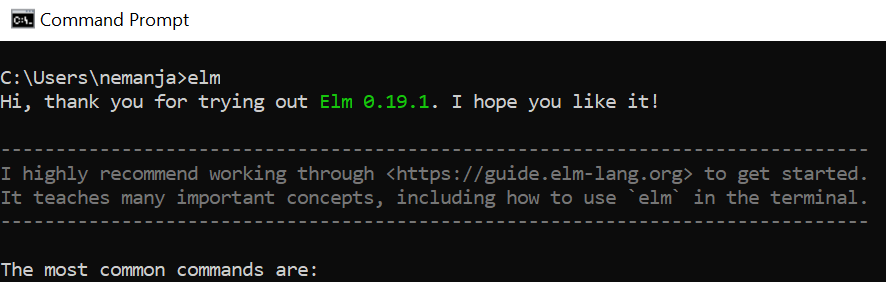
\includegraphics[width=0.95\textwidth]{elm-cmd.png}
  \caption{Elm - Cmd}
\end{figure}

Takođe, mooguća je instalacija pomoću \textbf{npm}
\footnote{Node Package Manager - JavaScript menadžer paketa} alata \cite{npm}.

\section{Osnovne odlike}
Pored \emph{No Runtime Exceptions}, jedna od glavnih odlika ovog jezika jeste
kompilator, koji je izuzetno ugodan za rad. Mnogi programeri smatraju da Elm
kompilator proizvodi najbolje poruke o greškama. Za razliku od drugih, Elm
kompilator objašnjava zašto je došlo do greške i daje predloge za njihovo rešavanje,
a takođe nema kaskadnih poruka. Kreator se vodio razmišljanjem da kompilator treba
da bude asistent, ne samo alat.

Elm koristi svoju verziju \emph{virtualnog DOM-a}, koncepta koji se koristi u mnogim
frontend okruženima. Ideja je da se u memoriji čuva "virtualna" reprezentacija
korisničkog interfejsa  na osnovu koje se ažurira "stvarni" DOM. Još jeda bitna
karakteristika Elm-a je nepromenjivost podataka, što znači da se jednom definisani
podaci ne mogu više menjati. Direkta posldica nepromenjivost podataka je veoma
brzo renderovanje HTML-a, jer se poređenja u virtuelnom DOM-u mogu vršiti po referenci. 
Verzija Elm 0.17 imala je najbrže renderovanje u poređenju sa tadašnjim aktuelnim verzijama 
popularnih okruženja.

Elm se može integrisati i u postojeće JavaScript projetke za implementaciju pojedinačnih 
komponenti. Takođe, moguća je i komunikacija između Elm-a i JavaScripta. 

\section{Elm kao platforma}
Elm sa sobom donosi niz alata (tabela \ref{table:1}) i Elm okruženje (\emph{eng. Elm 
Runtime}), koji su neophodni za razvoj i izvršavanje aplikacija. Elm kod se nalazi u 
datotekama sa \emph{.elm} ekstenzijom i prilikom kompilacije kreira se jedna izlazna 
\emph{.js} datoteka. U izlaznoj datoteci se pored prevedenog koda iz ulaznih \emph{.elm} 
datoteka nalaze i (runtime) funkcije iz Elm okruženja potrebne za izvršavanje programa.


\begin{table}[h!]
\centering
\begin{tabular}{|l l|} 
 \hline 
 Alati & Kratat opis  \\ [0.5ex] 
 \hline
  \textbf{repl} & Pokretanje interaktivne sesije (\emph{eng. Read-Eval-Print-Loop}) \\ 
  \textbf{init} & Inicijalizacija projekta \\
  \textbf{reactor} & Pokretanje lokalnog servera \\
  \textbf{make} & Upotreba kompilatora \\
  \textbf{install}  & Preuzimanje paketa \\ 
  \textbf{diff} & Prikazivanje razlika između različitih verzija istog paketa \\
  \textbf{bump} & Određivanje broja naredne verzije paketa  \\
  \textbf{publish} & Publikacija paketa \\[1ex] 
 \hline
\end{tabular}
\caption{Elm alati komandne linije}
\label{table:1}
\end{table}

 
Kao zaseban jezik Elm ima i zaseban sistem za upravljanje paketima.
Pokretanjem komande \textbf{elm init} kreira se prazan \emph{src} direktorijum i 
datoteka \emph{elm.json}, u kojoj se pored informacije o tipu projekta (aplikacija ili 
paket), Elm verzije i liste direktorijuma sa kodom, nalazi i spisak paketa koji se 
koriste u projektu. Dodavanje novog paketa se vrši pomoću komande \textbf{elm install} 
\emph{naziv-paketa}. Svi paketi nalaze se na \url{https://package.elm-lang.org/}, nazivi 
paketa su oblika \emph{autor/ime-paketa}.

Kompilacija se vrši naredbom \textbf{elm make} \emph{<jedna-ili-više-elm-datoteka>},
ukoliko se ne navede izlazna datoteka pomoću argumenta \emph{-{}-output} generisaće 
se \emph{index.html} datoteka sa prevedenim JavaScript kodom. Ostali argumenti ako i
više informacija o drugim alatima može se videti pomoću naredbe \textbf{elm} 
\emph{naziv-alata} \textbf{-{}-help}

\section{Elm kao jezik}
\begin{displayquote}
"Rekao bih da je Elm ML sa sintaksom poput Haskell-a. Ako poredimo semantiku, Elm je
dosta  sličniji OCaml-u i SML-u." \emph{--Evan Czaplicki \cite{eczaplicki:2015}} 
\end{displayquote}

\textbf{ML} (\emph{eng. Meta Language}) je statički tipiziran programski jezik opšte 
namene koji je razvio Robin Miler 1978. godine na Univerzitetu u Edinger. Nastao je pod 
uticajem LISP-a i ISWIM-a (\emph{eng. If you See What I Mean}) jezika, pripada 
funkcionalnoj i imperativnoj paradigmi. Neke od osnovnih karakteristika jesu poklapanje 
obrazaca, Karijeve funkcije, poziv po vrednosti i posedovanje sakupljača otpadaka. ML nije 
čist funkcionalan jezik i nema ugrađenu podršku za lenjo izračunavanje. U porodicu ML 
jezika, između ostalih, spadaju i \textbf{Standard ML}, \textbf{OCaml} i \textbf{F{\#}}.


\textbf{Haskell} je čist funkcionalni programski jezik zasnovan na lambda računu.
Naziv je dobio po matematičaru i logičaru Haskelu Bruks Kariju. Haskell je strogo 
tipiziran, poseduje automatsko zaključivanje tipova i lenjo izračunavanje. Jezik je 
opšte namene, pruža podršku za paralelno i distirbuirano programiranje. Haskell 
omogućava manje grešaka i veću pouzdanost kroz kraći, čistiji i održiviji kod.


\subsection{Osnovni tipovi podataka}
\begin{listing}[ht]
\begin{minted}[bgcolor=black]{haskell}
> 'Z'
'Z' : Char
> "Zdravo!"
"Zdravo!" : String
> True
True : Bool
>42
42 : number
> 42 / 10 
4.2 : Float
> 42 // 10 --celobrojno deljenje
4 : Int
\end{minted}
\caption{Osnovni tipovi podataka (elm repl)}
\label{listing:tipovi}
\end{listing}

Osnovni tipovi podataka u Elmu su \textbf{Char}, \textbf{String}, \textbf{Bool}, 
\textbf{Int} i \textbf{Float}. U Listingu \ref{listing:tipovi} prikazani su osnovni 
tipovi korišćenjem interpretera, budući da i Elm posedjue zaključivanje tipova, nakon 
izračunate vrednosti unetog izraza ispisuje se i tip. U konkretnom primeru broj 42 se 
može posmartati i kao \textbf{Int} i kao \textbf{Float}, pa interpreter vraća 
\texttt{number} kao tip, iako \texttt{number} nije tip podataka.


Tip \textbf{Char} služi za predstavljanje unikod (\emph{eng. unicode}) karaktera. 
Karakteri se navode između dva apostorfa (\texttt{'a', '0', '\textbackslash t'}...), a 
moguće je koristiti i unikod zapis  \texttt{'\textbackslash u\{0000\}}' - 
\texttt{'\textbackslash u\{10FFFF\}'}.

Za razliku od Haskell-a, gde je \textbf{String} zapravo \textbf{Char} lista, u Elmu je 
poseban tip i predstavlja sekvencu unikod karaktera. Sekvenca se navodi između 
jednostrukih ili trostrukih navodnika. 

\begin{listing}[ht]
\begin{minted}[bgcolor=black]{haskell}
> "\t String u jednom redu: escape navodnici \"Zdravo!\""
"\t String u jednom redu: escape navodnici \"Zdravo!\"" : String
>
> """String u više redova
 sa "navodnicima"! """
"String u više redova\n  sa \"navodnicima\"! " : String
\end{minted}
\caption{Stringovi}
\label{listing:string}
\end{listing}

\textbf{Bool} predstavlja logički tip i može imati vrednost \texttt{True} ili \texttt{False}. 

\textbf{Int} se koristi za prikazivanje celih brojeva. Siguran opseg vrednosti je 
od \(-2^{31}\) do \(2^{31} - 1\), van toga sve zavisi od cilja kopilacije. Kada se 
prevodi u JavaScript, opseg se proširuje na \(-2^{53}\) do \(2^{53} - 1\) u nekim 
operacijama, što ne bi važilo ukoliko bi se, nekada kasnije, umesto JavaScript koda 
generisao WebAssembly, tada bi postojalo prekoračenje celih brojeva(\emph{eng. integer 
overflow}). Vrednosti se mogu navoditi i u heksadecimalnom obliku  (\texttt{0x2A, -0x2b}).

\textbf{Float} služi za predstavljanje brojeva u pokretnom zarezu po strandardu 
\emph{IEEE 754}. Vrednosti se mogu navoditi i pomoću eksponencijalnog zapisa, a decimalna 
tačka se mora nalaziti između dve cifre. Takođe, u skup vrednosti spadaju \texttt{NaN} i 
\texttt{Infinity} (listing \ref{listing:brojevi}) .

\begin{listing}[ht]
\begin{minted}[bgcolor=black]{haskell}
> 1e3
1000 : Float
> 0/0 
NaN : Float
> 1/0 
Infinity : Float
\end{minted}
\caption{Brojevi u pokretnom zarezu}
\label{listing:brojevi}
\end{listing}

\subsection{Osnovni operatori}
Kod artimetičkih operacija, operatori \texttt{+, -, *} se mogu koristi sa realnim i 
celim brojevim, dok imamo posebne operatore za deljenje( \texttt{{/}} i \texttt{{//}}
- listing \ref{listing:tipovi}). Elm ne podržava implicitne konverzije tipova, pa
prilikom sabiranja celog broja sa realnim, bez eksplicitne konverzije, kompilator
prijavljuje grešku. Postoji još i eksponencijalni operator \^{}, a za celobrojno deljenje 
sa ostatkom koriste se funkcije \texttt{modBy} i \texttt{remainderBy}.
\begin{listing}[h]
\begin{minted}[bgcolor=black]{haskell}
> toFloat (9 // 3) + 3.2
6.2 : Float
> 9 // 3 + round 3.2
6 : Int
> 9 // 3 + 3.2 -- TYPE MISMATCH error
\end{minted}
\caption{Konverzija tipova}
\label{konverzija}
\end{listing}

Elm pruža \texttt{\&\&} i \texttt{||} logičke operatore kao i funkcije za negaciju 
\texttt{not} i ekskluzivno ili \texttt{xor}. Operator \texttt{\&\&} ima viši priotiter 
od \texttt{||}, oba su levo asocijativna i lenjo izračunljiva. Od operatora poređenja 
\texttt{==, /=, <, >, >= i <=} jedino operator različitosti (\texttt{/=}) ima drugačiju 
od uobičajene. Pored navednih, Elm podržava i \texttt{++} operator konkatenacije 
stringova i listi.

\begin{listing}[h]
\begin{minted}[bgcolor=black]{haskell}
> not (1 + 1 /= 2) && 2 + 2 <= 5 || 1^0 == 0^1 
True : Bool
> 2^6 - 0x100 / 4  * (1 + 2)
-128 : Float
> "Spojen " ++ "string!" == "Spojen string!"
True : Bool
\end{minted}
\caption{Operatori}
\label{konverzija}
\end{listing}

\subsection{Komentari}
Komentari se mogu navoditi na dva načina: \begin{itemize}
  \item Korišćenjem \texttt{-{}-} za linijske komentare
  \item Navođenjem teksta između \texttt{\{-} i \texttt{-\}} za komentare u više redova.    
\end{itemize}

\subsection{Funkcije}  
Sintaksa definisanje funkcija je veoma jednostavna i prikazana je u listingu 
\ref{listing:funkcije}.
\begin{listing}[h]
\begin{minted}[bgcolor=black]{haskell}
{-
  nazivFunkcije param1 param2 ... =
    izraz  
-}
deljivSa x y =
  modBy x y == 0

dobarDan x = "Dobar dan, " ++ x ++ "!"  
\end{minted}
\caption{Funkcije}
\label{listing:funkcije}
\end{listing}

Ime funkcije obavezno počinje malim slovom, nakon čega sledi niz slova (velikih i malih),
simbola \texttt{\textbf{\textunderscore}} i brojeva. Po konvenciji, sva slova se navode u
neprekidnoj sekvenci, stoga je preporučena kamilja notacija(\texttt{camelCase}).
Parametri se odvajaju razmakom, dok se zagrade ne navode ni prilikom definisanja, ni
pozivanja funkcije. Ipak, apikacija funkcije je levo asocijativna, pa je česta upotreba
zagrada za ograđivanje izraza. Telo funkcije predstavlja jedan jedini izraz koji se izvšava
prilikom pozivanja, a izračunata vrednost predstavlja povratnu vrednost funkcije. Ne koriste
se vitičaste zagrade, ni naredba \texttt{\textbf{return}}. Izraz se, po konvenciji, piše u
novom redu, ali je moguće i u istom\label{listing:funkcije}.

\subsubsection{Konstante}
U Elmu ne postoje promenljive, jednom definisani podaci se ne mogu promeniti, ali je 
moguće definisati konstante. Često se u literaturi definisanje konstanti naziva 
\emph{imenovanjem vrednosti izraza} i ne dovodi se u vezu sa funkcijama, ali se konstante 
mogu posmartati kao \emph{konstantne funkcije}, koje se izvrše tokom kompilacije. Definišu se
kao i funkcije, samo bez parametara \ref{listing:lambda}.

\subsubsection{Anonimne funkcije}
Anonimne funckije se definišu slično kao i regularne, umesto imena navodi se simbol 
\texttt{\textbf{\textbackslash}} koji predstavlja grčko slovo lambda - \(\lambda\),
dok se \texttt{\textbf{->}} koristi umesto znaka jednakosti \ref{listing:lambda}.
\begin{listing}[h]
\begin{minted}[bgcolor=black]{haskell}
> broj3 = 3
3 : number
> (\x y -> x + y) broj3 4
7 : number
\end{minted}
\caption{Primer anonimne funkcije}
\label{listing:lambda}
\end{listing}

Funkcije u Elmu mogu prihvatati funkcije kao parametre i vraćati funkcije kao 
povratne vrednosti, što ih čini funkcijama višeg reda. Nije moguće navoditi
podrazumevane vrednosti parametara, kao ni preopterećivanje funkcija.

\subsubsection{Moduli}
Moduli se koriste za grupisanje funkcija u logičke jedinice i kreiranje imenskih 
prostora(\emph{eng. namespace}). Svaki modul predstavlja jedanu \emph{.elm} datoteku,
koja se mora zvati isto kao i modul, dok ime modula mora počinjati velikim slovom.
Za definisanje modula koristi se ključna reč \texttt{\textbf{module}} nakon koje sledi
ime modula, ključna reč \texttt{\textbf{exposing}} i lista funkcija kojima se može 
pristupiti van modula.
\begin{listing}[h]
\begin{minted}[bgcolor=black]{haskell}
module Krug exposing (povrsina, obim) 
-- module Krug exposing (..) - otrkivanje svega iz modula 
pi = 3.14

povrsina r =
    naKvadrat r * pi

obim r =
    2 * r * pi

naKvadrat x =
    x * x
\end{minted}
\caption{Primer modula}
\label{listing:modul}
\end{listing}

Da bi se modul iz listinga \ref{listing:modul} koristio u \texttt{repl}-u, prvo je 
potrebno inicijalizovati elm projekat (\emph{elm init}) i u src folderu napraviti 
\emph{Krug.elm} datoteku sa prikazanim sadržajem. Zatim, u \texttt{repl}-u naredbom 
\texttt{\textbf{import}} uvesti modul. Načini korišćenja funkcija iz modula
\emph{Krug} prikazani su u listingu \ref{listing:import}.
\begin{listing}[h]
\begin{minted}[bgcolor=black]{haskell}
import Krug                           -- Krug.obim Krug.povrsina
import Krug as K                      -- K.obim K.povrsina

import Krug exposing (obim)           -- obim, Krug.povrsina
import Krug exposing (..)             -- obim, povrsina
import Krug as K exposing (povrsina)  -- K.obim, povrsina
\end{minted}
\caption{Primer korišćenja modula}
\label{listing:import}
\end{listing}

\subsubsection{Tip funkcije}
Prilikom definisanje funkcije u \texttt{repl}-u ili poziva funkcije bez parametara,
interpreter kao vrednost izraza vraća \texttt{\textbf{<function>}} i tip funkcije.
U listing-u  \ref{listing:tipoviFunkcije} prikazano je nekoliko primera tipova 
funkcija u \texttt{repl}-u.
\begin{listing}[h]
\begin{minted}[bgcolor=black]{haskell}
> not
<function> : Bool -> Bool
> deljivSa
<function> : Int -> Int -> Bool
> \x y z -> x + y + z
<function> : number -> number -> number -> number
> deljivSa 3 --parcijalna aplikacija
<function> : Int -> Bool
\end{minted}
\caption{Tipovi funkcija}
\label{listing:tipoviFunkcije}
\end{listing} 
  
U pirmeru funckije \texttt{\textbf{not}} vidimo da je njen tip \emph{Bool -> Bool},
što je dovoljno samorazumljivo i znači da se radi o funkciji jednog argumenta koja
prihvata vrednost tipa \emph{Bool} i vraća vrednost tipa \emph{Bool}. U slučaju
funkcija koje imaju više argumenata, tip funkcije ne mora biti toliko jasan i može 
se posmartati na način da poslednji tip u nizu razdvojenim strelicama
(\texttt{\textbf{->}}) predstavlja povrati tip funkcije, dok tipovi pre njega 
predstavljaju tipove argumenata funkcije. Postavlja se pitanje zašto se i tipovi 
argumenata međusobom odvajaju strelicama. Razlog za to su Karijeve (\emph{Curried})
funkcije u Elmu, što znači da su sve n-arne funkcije zapravo funkcije jednog argumeta
koje kao povratnu vrednost imaju funkciju.
\begin{figure}[!h]
  \centering
  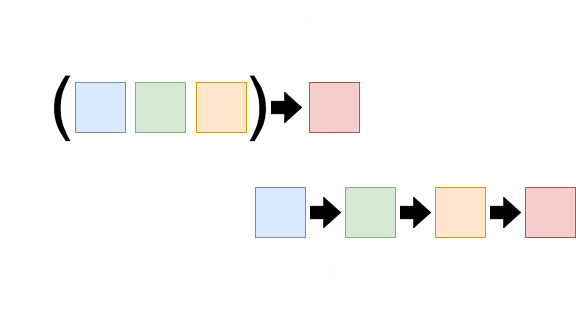
\includegraphics[width=0.5\textwidth]{currying.png}
  \caption{Regularne i Karijeve funkcije}
\end{figure}
Strelica(\texttt{\textbf{->}}) je desno asocijativna, a zagrade se izostavljaju zbog
jendostavnosti. Tako da funkcija \texttt{deljivSa} ima tip \emph{Int -> (Int -> Bool)},
što znači da prihvata vrednost tip \emph{Int} i vraća funkciju tipa \emph{Int -> Bool}.
Karijeve funkcije nam omogućavaju veću fleksibilnost i parcijalnu aplikaciju funkcija, 
odnosno vezivanje argumenata za konkretne vrednosti \ref{listing:tipoviFunkcije}.

\subsubsection{Anotacija tipa funkcije}
Kao što je prethodno prikazano, Elm sam zaključuje tip funkcije, ali dozvoljava i korisniku
da sam navede tip u liniji iznad definicije.
\begin{listing}[!h]
\begin{minted}[bgcolor=black]{haskell}
> deljivSa: Int -> Int -> Bool
| deljivSa x y =
|   modBy x y == 0
|
<function> : Int -> Int -> Bool
\end{minted}
\caption{Anotacija tipa funkcije}
\end{listing}

Korišćenje anotacije tipova nije obavezno, ali je vrlo preporučiljivo iz više razloga.
Prilikom kompilacije proverava se poklapanje anotacije sa stvarnim tipom funkcije, što
dovodi do lakšeg uočavanja i otklanjanja grešaka. Pored toga, anotacije predsavljaju veoma
dobar vid dokumentacije, a činjenica da kompilator uvek poredi navedeni i stvarni tip nam
garantuje da je dokumentacija uvek važeća.

\subsubsection{Funkcijski operatori}
Operatore nad funkcijama možemo podeliti prema tipu, na operatore prosleđivanja i operatore
kompozicije funkcija, i prema smeru u kom se primenjuju, unapred ili unazad.

Operatori prosleđivanja ili \textbf{pipe} operatori su zapravo operatori aplikacije funkcije
i omogućavaju pisanje čitljivijeg koda sa manje zagrada.
\begin{itemize}
  \item \texttt{\textbf{<|}} - pipe operator unazad radi isto što i aplikacija funkcije, 
  stim što nas oslobađa pisanja zagrada. Tako da je \texttt{\textbf{ f <| x}} identično
  \texttt{\textbf{ f (x)}}
  \item \texttt{\textbf{|>}} - pipe operator inspirisan je Unix pipe-om, odatle i
  naziv, i služi za prosleđivanje argumenta funkciji. \texttt{\textbf{ x |> f}} je zapravo
  \texttt{\textbf{ f (x)}}
\end{itemize}

Operator kompozicije unazad \texttt{\textbf{<<}} zapravo predstavlja operator matematičke 
kompozicije funkcija \(\circ\). Tako da se definicija kompozicije \((g \circ f)(x) = g(f(x))\)
u Elmu može posmatrati kao: \texttt{\textbf{(g << f) x == (\textbackslash x\textunderscore ->
g ( f x\textunderscore)) x}}. Dok je operator kompozicije \texttt{\textbf{>>}} obrnut i
simetričan je operatoru \texttt{\textbf{<<}} -- \texttt{\textbf{(f << g) x == (g >> f) x}}.

\subsection{Osnovne strukture podataka}
\subsubsection{Liste}
Lista u Elmu predstavlja kolekciju u obliku jednostruko povezane liste. Elementi se navode
unutar uglastih zagrada - \textbf{\texttt{[ ]}} i moraju biti istog tipa. Funkcije za rad
sa listama nalaze se unutar \texttt{List} modula. Pored operatora za nadovezivanje, postoji
i operator \texttt{::} koji dodaje element na početak liste. 
\begin{listing}[h]
\begin{minted}[bgcolor=black]{haskell}
> "aaa" :: ["bbb","ccc"]
["aaa","bbb","ccc"] : List String
> List.map (List.member 2) [[1,2,3],[2,2],[42]]
[True,True,False] : List Bool
> [1,2]++[3,4,5] |> List.filter (\x -> modBy 2 x == 0) |>List.length
2 : Int
> List.foldl (\x y -> x + y) 0 <| List.range 1 5 
15 : Int
\end{minted}
\caption{Liste}
\label{listing:liste}
\end{listing}
\subsubsection{Torke} 
Za razliku od listi koje mogu imati promenljivi broj elemenata istog tipa, torke 
predstavljaju kolekcije fiksne dužine čiji elementi ne moraju biti istog tipa. 
Mogu sadržati samo dva ili tri elementa, navode se unutar običnih zagrada -
\textbf{\texttt{()}} i ne mogu se ubacivati ili uklanjati elementi. Funkcije nad
torkama koje imaju dva element nalaze se u modulu \texttt{Tuple}.
\begin{listing}[h]
\begin{minted}[bgcolor=black]{haskell}
> (1,"2",'3')
(1,"2",'3') : ( number, String, Char )
> (1,2) == Tuple.pair 1 2
True : Bool
> Tuple.second ("nebitan", "drugi")
"drugi" : String
> Tuple.mapFirst String.length  ("mapiran", 1)
(7,1) : ( Int, number )
\end{minted}
\caption{Torke}
\label{listing:torke}
\end{listing}
\subsubsection{Rekordi} 
Rekord predstavlja strukuru podataka koja može sadržati više vrednosti različitih tipova, 
pri čemu je svakoj vrednosti dodeljen naziv. Liče na objekte u JavaScript-u, čak je i 
sintaksa veoma slična, umesto dvotačke rekord koristi znak jednakosti za dodelu naziva.
Prilikom definisanja rekorda, Elm kreira funkcije za pristup svojstvima rekorda. Nije 
moguće dodavanje, ni uklanjanje svojstava, ali je dozvoljena promena njihovih vrednosti.
Zbog imutabilnosti, ne vrši se promena nad postojećim rekordom već se pravi novi.
\begin{listing}[h]
\begin{minted}[bgcolor=black]{haskell}
> pera = {ime = "Pera", prezime = "Perić", godine = 23}
{ godine = 23, ime = "Pera", prezime = "Perić" } 
  : { godine : number, ime : String, prezime : String }
> {pera | prezime = "Petrović", godine = 24}
{ godine = 24, ime = "Pera", prezime = "Petrović" }
  : { godine : number, ime : String, prezime : String }
> pera.ime
"Pera" : String
> .godine pera
23 : number
> .prezime
<function> : { b | prezime : a } -> a
\end{minted}
\caption{Rekord}
\label{listing:rekord}
\end{listing}

Pored navedenih struktura podataka, Elm pruža podršku za rad sa nizovima (\texttt{Array}),
skupovima(\texttt{Set}) i rečnicima(\texttt{Dict}).

\subsection{Tipske promenljive} 
U listingu \ref{listing:rekord} vidimo da funkcija za pristup prezimenu ima tip:\\ 
\texttt{\textbf{\{ b | prezime : a \} -> a}}. Ovo znači da funkcija kao argumenat
prima rekord, koji može biti bilo kog tipa, ali mora imati svojstvo\texttt{\textbf{
prezime}}, koje takođe može biti bilo kog tipa, i čiji tip je ujedno povrati tip 
funkcije. Promenljive \texttt{\textbf{a}} i \texttt{\textbf{b}} nazivaju se 
\emph{tipske promenljive}, a prisustvo dve tipske promenljive nam govori da one mogu, 
ali ne moraju, predstavljati različite tipove. U konkretnom primeru \texttt{\textbf{a}}
i \texttt{\textbf{b}} su uvek različitog tipa, dok u slučaju funckije \texttt{Tuple.pair
: a -> b -> ( a, b )} mogu biti istog tipa. Prilikom anotacije tipova mogu se koristi i
duža imena tipskih pormenljivih, a pravlia imenovanja su ista kao i za funkcije.

Tipske promenljive u Elmu ukazuju na prisustvo \textbf{parametarskog polimorfizma},
jedine vrste polimorfizma u ovom jeziku.

\subsubsection{Uslovne tipske promenljive}
Za razliku od Haskell-a, Elm nema toliko složen sistem tipova i umesto tipskih klasa
(\emph{eng. typeclasses})\cite{typeclasses} poseduje jednostavniji koncept --
\emph{uslovne tipske promenljive}. 

Uslovne tipske promenjljive omogućavaju da se na određni način ograniči skup tipova
koji se može koristiti u izrazima. Najčešći primer je \texttt{number}, koji dozvoljava 
isključivo \texttt{Int} ili \texttt{Float} tipve. 

U trnutnoj verziji(\emph{0.19.1}) postoje četiri uslovne tipske promenjljive:
\begin{enumerate}
  \item \texttt{number} - dozvoljava \texttt{Int} i \texttt{Float}
  \item \texttt{appendable} - dozvoljava \texttt{String} i \texttt{List a}
  \item \texttt{comparable} - dozvoljava \texttt{Int}, \texttt{Float}, \texttt{Char},
  \texttt{String}, liste i torke koje sadrže \texttt{comparable} vrednosti
  \item \texttt{compappend} - dozvoljava \texttt{String} i \texttt{List comparable}
\end{enumerate}

\subsubsection{Operatori i tipske promenljive}
\begin{listing}[h]
\begin{minted}[bgcolor=black]{haskell}
> (+) 1 2
3 : number
> (*)
<function> : number -> number -> number
> (++)
<function> : appendable -> appendable -> appendable
> (==)
<function> : a -> a -> Bool
> (>=)
<function> : comparable -> comparable -> Bool
\end{minted}
\caption{Uslovne tipske promenljive}
\label{listing:tipskePromenljive}
\end{listing}
Operatori u Elmu predstavljaju funkcije koje se mogu pozivati u infiksnoj notaciji. Takođe, 
mogu se pozivati i u prefiksnoj ukoliko ih navedemo unutar zagrada: \texttt{\textbf{(+),
(++), (>=)}}... , dok pozivanjem bez argumenata možemo videti i kog su tipa.

U ranijim verzijama jezika bilo je moguće definisati korisničke operatore, ali je ta
opcija izbačena u verziji 0.19.0., a od verziji 0.18.0 nije moguće pozivanja 
binarnih funkcija u infiksnoj notaciji.

\subsection{Aliasi tipova}
Prilikom definisanja funkcija koje rade nad istim strukturama podataka višestruko navodimo
iste anotacije tipova, pritom anotacije podataka mogu biti predugačke, samim tim i
teško čitljive. Aliasi tipova nam omogućavaju ponovnu upotrebu anotacija i bolju čitljivost.
Definišu se pomoću ključnih reči \texttt{\textbf{type alias}}, nakon kojih sledi ime koje
mora počinjati velikim slovom. 
\begin{listing}[h]
\begin{minted}[bgcolor=black]{haskell}
>type alias MatricaInt3 = List (List (List Int))
>
>type alias Osoba = {ime : String, prezime : String, godine : Int }
> Osoba
<function> : String -> String -> Int -> Osoba
> Osoba "Pera" "Perić" 23
{ godine = 23, ime = "Pera", prezime = "Perić" } : Osoba
\end{minted}
\caption{Aliasi tipova}
\label{listing:alias}
\end{listing}

Prilikom kreiranja aliasa za rekord kreira se i konstruktor za rekord, što se može videti
u listingu \ref{listing:alias}. Redosled argumenata funkcije za konstrukciju identičan je
redosledu u aliasu.
\subsection{Korisnički definisani tipovi}
Pored korišćenja aliasa za postojeće tipove podataka, Elm pruža mogućnost kreiranja novih 
tipova. Korisnički definisani tipovi se često nazivaju i\emph{unijski tipovi}, jer mogu  
predstavljati uniju više varijanti definisanog tipa. Definišu se ključnom reči 
\textbf{\texttt{type}}, a varijante se odvajaju simbolom \texttt{\textbf{|}}.

Slično kao kod aliasa tipova za rekorde i ovde se kreiraju konstruktori za definisani tip. 
\begin{listing}[h]
\begin{minted}[bgcolor=black]{haskell}
> type VectorF4 = Vector4F Float Float Float Float
> Vector4F
<function> : Float -> Float -> Float -> Float -> VectorF4
>
>type StatusPrijave 
  = NaCekanju 
  | Greska String 
  | Uspesno {id : Int, token : String}
> NaCekanju
NaCekanju : StatusPrijave
> Greska
<function> : String -> StatusPrijave
> Uspesno
<function> : { id : Int, token : String } -> StatusPrijave
\end{minted}
\caption{Korisnički definisani tipovi}
\end{listing}

\subsection{Kontorla toka}
U Elmu nema izvršavanja naredbi, već samo evaluacije izraza, tako da umesto naredbi grananja
imamo \texttt{\textbf{if}} i \texttt{\textbf{case}} izraze, a rekurziju umesto petlji.  
\subsubsection{If izraz}
\texttt{\textbf{if}} izraz se može posmatrati kao ternarni operator u JavaScript-u, C++-u i 
mnogim drugim programskim jezicima.
\begin{listing}[h]
\begin{minted}[bgcolor=black]{haskell}
{-    uslov   ?  izraz1   :  izraz2   - ternarni operator
   if uslov then izraz1 else izraz2   - if izraz
-}
if x >= 0 then "pozitivan" else "negativan"
if x == 1 then x * 2 else if x == 2 then x / 2 else x
\end{minted}
\caption{If izraz}
\label{listing:if}
\end{listing}

Ključna reč \texttt{\textbf{else}} je sastavni deo \texttt{\textbf{if}} izraza tako
da \texttt{\textbf{else}} "grana" uvek postoji. Mogu se navoditi i ugnježdeni
\texttt{\textbf{if}} izrazi, pa \texttt{\textbf{else if}} grana predstavlja korišćenje
\texttt{\textbf{if}} izraza nakon ključna reč \texttt{\textbf{else}}.

\subsubsection{Case izraz}
Izraz \texttt{\textbf{case}} predstavlja pandan \texttt{\textbf{switch}} naredbi u drugim
programski jezicima. Mogu da rade samo nad jednim tipom vrednosti, a prilikom korišćenja 
\texttt{\textbf{case}} izraza moraju se pokriti sve mogućnosti. Za podrazumevani slučaj 
može se korisiti simbol \texttt{\textbf{\textunderscore}}. \texttt{\textbf{Case}} izrazi 
zauzimaju značajno mesto u Elmu, jer se koriste u \textbf{poklapanu obrazaca}.
\begin{listing}[h]
\begin{minted}[bgcolor=black]{haskell}
case mesto of
  1 -> "zlato"
  2 -> "srebro"
  3 -> "bronza"
  _ -> "zahvalnica"
\end{minted}
\caption{If izraz}
\label{listing:case}
\end{listing}
\subsubsection{Let izrazi}
Budući da ne postoje blokovi naredbi, \texttt{\textbf{let}} izrazi nam omogućavaju da 
ograničimo oblast važenja - \emph{ dosega (eng. scope)} funkcija i konstanti u okviru
jedne funkcije. Doprinose boljoj čitljivosti koda, a moguće je koristiti anotacije tipova
unutar njih.
\begin{listing}[h]
\begin{minted}[bgcolor=black]{haskell}
let
  nula: Int
  nula = 0
  
  pozitivan: Int -> Bool
  pozitivan =
    \x -> x > nula
in pozitivan 10
\end{minted}
\caption{Let izraz}
\end{listing}
\subsubsection{Rekurzija}
Rekurzivno definisana funkcija poziva samu sebe, čime se postiže ponavljanje koje imamo
korišćenjem petlji. U nekim slučajevima, umesto rekurzije mogu se koristiti funkcije nad
listama.
\begin{listing}[h]
\begin{minted}[bgcolor=black]{haskell}
factorial n = 
  if n <= 1 then 1 
  else  n * factorial (n - 1)

factorialFold n = 
  List.foldl (*) 1 (List.range 1 n) 
\end{minted}
\caption{Rekurzija}
\end{listing}

\subsection{Poklapanje obrazaca}
Poklapanje obrazaca može se posmatrati kao pokušavanje usklađivanja(poklapanja) ulaznog
podatka sa unapred definisanim obrascom. Ukoliko dođe do usklađivanja, poklopljenim
vrednostima se može prisupiti putem identifikatora definisanim u obrascu. Pored spomenutih
\texttt{\textbf{case}} izraza, u Elmu se poklapanje obrazaca može korisiti u vidu 
destrukcije rekorda ili torki prilikom definisanja funkcija ili korišćenja\texttt{\textbf{
let}} izraza.
\begin{listing}[h]
\begin{minted}[bgcolor=black]{haskell}
-- liste 
case lista of
  [] -> "prazna lista"
  [_] -> "jedan element"
  [a,b] -> "dva elementa:" ++ a ++ " i " ++ b
  a :: _ -> "više od dve elemenata, prvi je: " ++ a

-- unijski tipovi
case prijava of
  NaCekanju -> "Molimo za strpljejne"
  Greska poruka -> "Došlo je do grške: " ++ poruka
  Uspesno {id} -> "Uspešna prijava, id: " ++ String.fromInt id

-- torke
case tacka3D of
  (0, 0, 0) -> "centar"
  (0, _, _) -> "na x-osi"
  _ -> "van x-ose"

-- destrukcija
let
  (x,_,_) = tacka3D
in "x koordinata je " ++ String.fromFloat x

--nije moguće poklapanje ugnježdenih rekorda
prikaziPodatke ({ime, adresa} as osoba) =
  ime ++ " " ++ osoba.prezime ++ " " ++ adresa.ulica
\end{minted}
\caption{Poklapanje obrazaca}
\label{listing:pokalapanjeObrazaca}
\end{listing}

Unutar case izraza sekvencijalno se vrši poklapanje obrazaca. Kada dodje do poklapanja
izračunava se izraz dodeljen datom obrascu, ne nastavlja se sa poklapanjem. Kompilator
prepoznaje ukoliko može doći do nepoklapanja nijednog obrasca i prijavljuje grešku.
Takođe, greška se prijavljuje i ukoliko se navede redudantan obrazac, tj. obrazac čiji je
skup vrednosti zapravo podskup skup vrednosti prethodno definisanog obrasca. 
Simbol \texttt{\textbf{\textunderscore}} služi za poklapanje vrednosti koje se ne koriste,
a ključna reč \texttt{\textbf{as}} se može koristiti ukoliko je potrebno pristupiti celom
ulaznom podatku. U listingu \ref{listing:pokalapanjeObrazaca} mogu se videti primeri
poklapanja obrazaca.

\subsection{Maybe i Result}
U Elmu ne postoje \texttt{\textbf{undefined, null, nil}} i ostale slične vrednost prisutne
u drugim programskim jezicima. Umesto njih koriste se \texttt{\textbf{Maybe}} i
\texttt{\textbf{Result}} koji potiču iz Haskell-a, gde imamo \texttt{\textbf{Maybe}} i
\texttt{\textbf{Either}}.

\subsubsection{Maybe}
Ukoliko bismo želeli da napišemo funkciju koja vraća prvi element liste, u slučaju da on
postoji vratili bismo \textbf{baš} njega. Ali šta bismo vratili ukoliko je lista prazna?
Pa \textbf{ništa}. Srećom, funkcija \texttt{List.head : List a -> Maybe a} radi upravo to
pa ne moramo da je pišemo i ukoliko je pozovemo \textbf{možda} name vrati prvi element.

\texttt{\textbf{Maybe}} se definiše kao \texttt{\textbf{type Maybe a = Just a | Nothing}}
i može se koristit za opcione argument, obradu grešaka i u rekordima sa opcionim svojstvima.
Zapravo svuda gde očekivani podatak može, ali ne mora, postojati.

\subsubsection{Result}
Za razliku od \texttt{\textbf{Maybe}}, koji bi u slučaju greške vratio \texttt{
\textbf{Nothing}}, \texttt{\textbf{Result}} nam daje mogućnost pružanja dodatnih 
informacija o grešci. Definiše se na sledeći način: \begin{tabbing}
\texttt{\textbf{type}} \= \texttt{\textbf{ Result error value}} \\
\> \=  \texttt{\textbf{= Ok value}} \\\>
\> \texttt{\textbf{| Err error }}
\end{tabbing}

\section{Elm arhitektura}

\chapter{Razvojno okruženje Phoenix i Elixir}

\chapter{Implementacija MSNR portala}

% ------------------------------------------------------------------------------
\chapter{Zaključak}
% ------------------------------------------------------------------------------


% ------------------------------------------------------------------------------
% Literatura
% ------------------------------------------------------------------------------
\literatura

% ==============================================================================

\end{document}